\documentclass[aspectratio=169,8pt]{beamer}
\setbeamercolor{frametitle}{fg=black,bg=white}
\setbeamertemplate{frametitle}
{\begin{centering}\smallskip
    \insertframetitle\par
    \smallskip\end{centering}}
\setbeamertemplate{itemize item}{$\bullet$}
\setbeamertemplate{navigation symbols}{}

\setbeamertemplate{navigation symbols}{}
\setbeamertemplate{caption}{\raggedright\insertcaption\par}

\newcommand{\topline}{%
  \begin{tikzpicture}[remember picture,overlay]
   \node[xshift=0.5\paperwidth,yshift=-1cm] at (current page.north west){%
    
\includegraphics[width=\paperwidth]{i/line.png}};
  \end{tikzpicture}
}

\long\def\bframe#1#2\eframe{\begin{frame}{#1}\topline#2\end{frame}}
\long\def\bbframe#1\eframe{\begin{frame}#1\end{frame}}
\long\def\be#1\ee{\begin{align*}#1\end{align*}}
\long\def\bcc#1\ecc{\begin{columns}#1\end{columns}}
\long\def\bc#1\ec{\begin{column}{0.48\textwidth}#1\end{column}}
\newcommand{\fig}[1]{%
  \begin{center}
    \includegraphics[width=\textwidth]{#1}
\end{center}}
\newcommand{\wfig}[2]{%
  \begin{center}
    \includegraphics[width=#1\textwidth]{#2}
  \end{center}}
\newcommand{\ffig}[2]{%
    \includegraphics[width=#1\textwidth]{#2}}

\usepackage{tikz}
\usepackage{helvet}
%\usepackage[export]{adjustbox}
%\usepackage{makecell}


\begin{document}
\bframe{Aphros}
``Sea-Foam''
\begin{center}
  
\includegraphics[width=0.5\textwidth]{i/god.png}
\end{center}
\eframe

\bframe{Aphros}
\begin{center}
  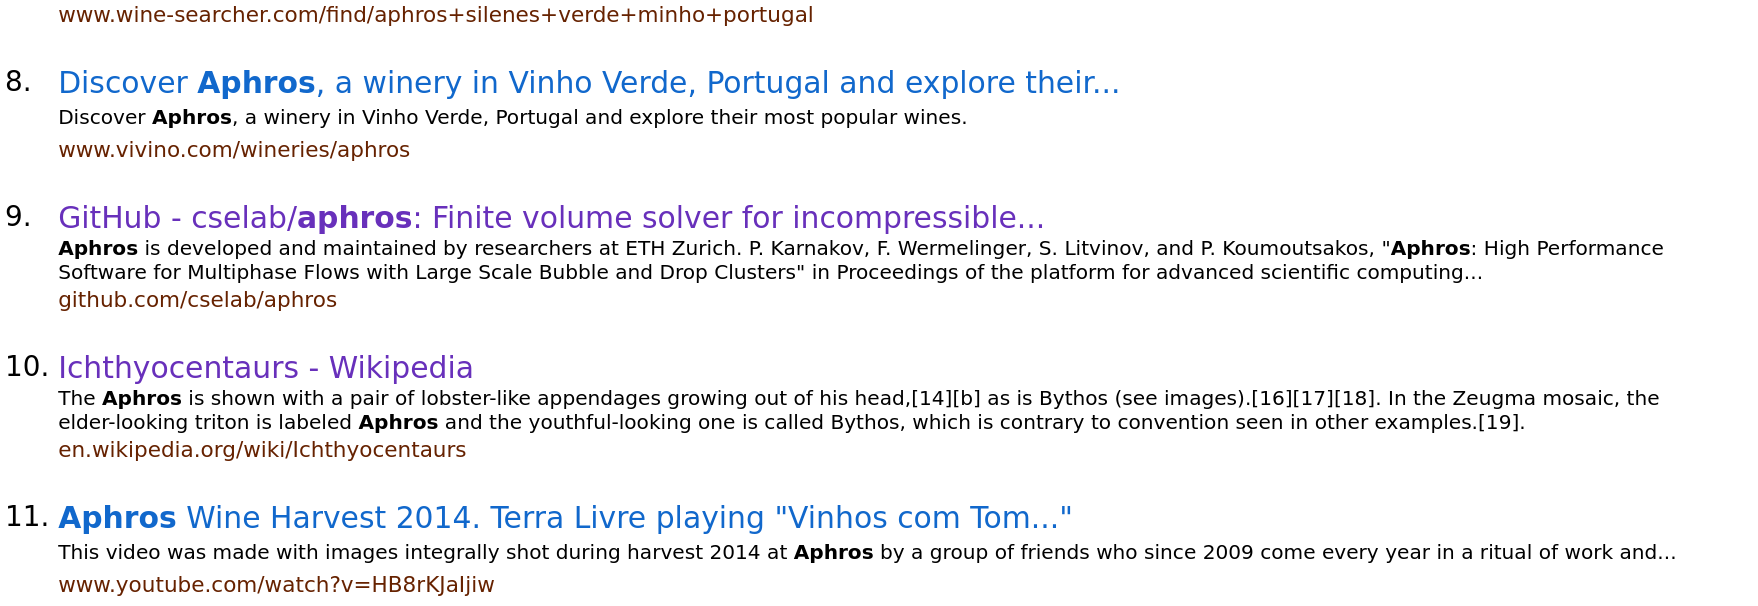
\includegraphics[width=0.75\textwidth]{i/ddg.png}
\end{center}
\eframe

\bframe{Authors}
\\
Petr Karnakov\\
Sergey Litvinov\\
Fabian Wermelinger\\
Prof. Petros Koumoutsakos
\vskip 4em
Based on Cubism: \\
D. Rossinelli, B. Hejazialhosseini, P. Hadjidoukas, C. Bekas, A. Curioni, A. Bertsch, S. Futral, S. J. Schmidt, N.A.~Adams, U. Rasthofer, J. Sukys, C. Conti., M. Chatzimanolakis, I. Kičić
\eframe

\bframe{Innovations}

- coroutines for block-wise processing
framework \\
\bigskip
- a particle method for curvature estimation \\
\bigskip
- coalescence prevention

\eframe

\bframe{Feedback}

rotoshake(r/vfx): Make an egg cream. I’ve seen good foam simulations
before but not being generated right out of the fluid like
that. Impressive.

\bigskip

ValarDohaerys(r/CFD): Really cool! I'm preparing for my fluid mechanics 2 exam these days and I can kind of keep up with the maths and modeling. Wohoo, nice to see that all the stuff pays off and is actually used. I find the example especially interesting (chemEng).
Just needed to nerd-talk. Sry for that xD

\bigskip

s-macke(HN): Two-phase fluid flow with surface tension in the
web. Fantastic! I tried it myself, but my simulations most of the time
exploded .... I mean diverged.  Keep up the good work! Presenting the
research is a must and thanks to cross compilers and WebAssembly it
was never so easy to even demonstrate your simulation code.

\eframe

\bframe{Outlook}

- dynamic contact line \\
\bigskip
- models for coalescence \\
\bigskip
-(adaptive) multi-resolution \\
\eframe

\end{document}
